\chapter{Processamento de Imagens}

O processamento digital de imagens é um campo cujas aplicações são bastante extensas. Existem métodos de processamento de imagens para interesses muito diferentes, que vão desde a melhoria das informações visuais para a interpretação dos médicos até a computação dos dados da imagem para transmissão, armazenamento ou interpretação autônoma por computador \cite{gonzalez}.

O processamento digital de imagens médicas é uma área em grande evolução e uma das que mais representa desafios dentro do processamento de imagens. Mas apesar de ser objeto de pesquisas de várias instituições ao redor do mundo, são poucos os sistemas deste tipo utilizados na prática médica. O principal fator é que este tipo de sistema exige alta eficiência, pois deve ser rápido, para que o tempo de resposta ao paciente não seja grande e ter uma baixíssima taxa de erros. Seus resultados são utilizados para tomar decisões em termos de diagnóstico e escolha de tratamento, por isso, alguns tipos de erro são inadmissíveis.

Em geral, os sistemas de processamento de imagens médicas extraem informações que podem ser provenientes de diversos tipos de modalidades de imagens, como Radiografia, Ultra-sonografia e Ressonância Magnética Nuclear, entre outras. Além das técnicas de processamento de imagens, técnicas de inteligência artificial, reconhecimento de padrões, entre outras áreas computacionais, são também aplicadas com o objetivo de melhorar tais imagens e extrair delas informações úteis ao diagnóstico.

\section{Imagens de tomografia computadorizada}

A tomografia era um dos mais importantes métodos de diagnóstico radiológico até a invenção da tomografia computadorizada - TC, na década de 70 do século passado. Sendo um dos primeiros tipos de exame a se beneficiar da popularização da computação.

A utilização de imagens no campo da medicina tem como principal objetivo proporcionar uma avaliação não invasiva dos tecidos e órgãos do corpo humano, tornando possível a verificação de anormalidades cautilizadas por doenças ou acidentes \cite{oliveira}.

As máquinas de TC possuem uma fonte de raios x e detectores de raios x, os quais ficam em lados opostos um do outro. Para construir as imagens de TC a fonte e os detectores de raios x são movidos para posições pre-determinadas e então obtem diversas imagens, como demonstrado na fig.~\ref{fig:tc1}, as quais representam fatias finas do paciente.

\begin{figure}[ht]
 \begin{center}
  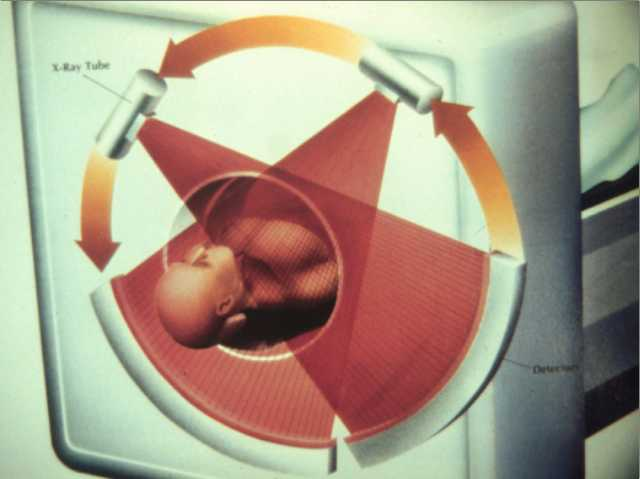
\includegraphics{imagens/tc.jpg}
 \end{center}
 \caption[Demonstração de como uma máquina de TC obtém as fatias de imagem do paciente.]{Demonstração de como uma máquina de TC obtém as fatias de imagem do paciente.\\* \\* Fonte: \citealt{sprawls}}
 \label{fig:tc1}
\end{figure}

A forma de movimentação depende da tecnologia da máquina utilizada. Nas máquinas mais antigas, eram tiradas várias projeções de uma fatia do paciente, apenas circulando em torno dele, e então depois a "cama" onde o paciente deita-se se move, para outra rodada de projeções, como na fig.~\ref{fig:tc2}. Hoje em dia, temos as máquinas helicoidais, os quais descrevem uma hélice em torno do paciente, em vez de uma sucessão de círculos completo. Desta forma é obtida informação de uma forma contínua.

\begin{figure}[ht]
 \begin{center}
  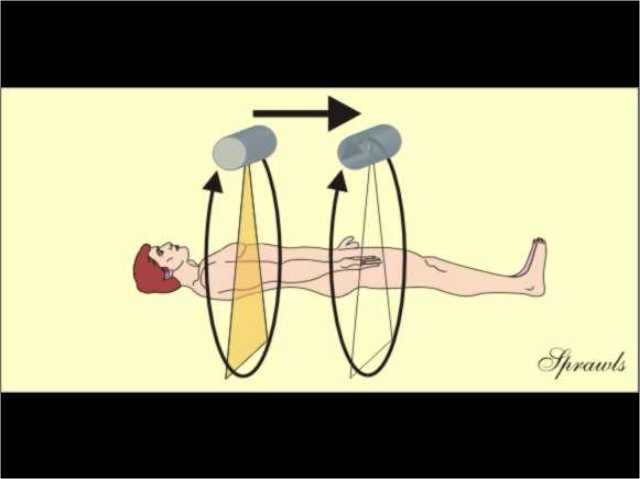
\includegraphics{imagens/tc2.jpg}
 \end{center}
 \caption[Forma de movimentação de máquinas de TC de tecnologia antiga.]{Forma de movimentação de máquinas de TC de tecnologia antiga.\\* \\* Fonte: \citealt{sprawls}}
 \label{fig:tc2}
\end{figure}

O resultado de cada pixel das fatias obtidas é a soma das energias bloqueadas pelos tecidos do corpo, e sabe-se exatamente em que ângulo cada fatia foi tirada, por isso após a aquisição das seções transversais, é possível a reconstrução da imagem em até 3 dimensões. Para a reconstrução é utilizada uma técnica matemática chamada de projeção retrógrada, ou outras, como a transformada de Fourier.

O campo de visão de uma imagem de TC representa o tamanho máximo do objeto em estudo que ocupa a matriz de pixels, por exemplo, uma matriz 512x512 pixels, se ela possuir um campo de visão de 12cm, cada pixel vai representar cerca de 0,023cm. Assim para o estudo de estruturas delicadas, como o ouvido interno, o campo de visão é pequeno, enquanto que para o estudo do abdômen o campo de visão é maior, em torno de 50cm (se tiver uma matriz de 512x512, então o tamanho da região que cada pixel representa vai ser próximo de 1 mm) \cite{tomo}.

\subsection{Coeficiente de Hounsfield}

A escala da unidade hounsfield - UH - é uma transformação linear da medida do coeficiente de atenuação linear original, do qual a radiodensidade da água destilada a temperatura e pressão ambientes é definida como 0 UH, enquanto a radiodensidade do ar a temperatura e pressão ambientes é -1000 UH. Para um material X com coeficiente de atenuação $\mu$X, o correspondente valor em unidades Hounsfiled é dado por:

\begin{equation}
	\frac{\mu_X-\mu_{H_2O}}{\mu_{H_2O}-\mu_{ar}}\times 1000
\end{equation}

onde $\mu_{H_2O}$ e $\mu_{ar}$ são os coeficientes de atenuação linear da água e do ar, respectivamente, a pressão e temperatura ambientes. Então uma mudança de uma UH representa uma mudança de 0,1\% da diferença do coeficiente de atenuação entre a água e o ar, ou aproximadamente 0,1\% do coeficiente de atenuação da água, já que o coeficiente de atenuação do ar é aproximadamente 0. Alguns valores Hounsfield conhecidos estão mostrados na tab.~\ref{tab:hounsfield}.

\begin{table}
 \caption{Valores Hounsfield comuns.}
 \begin{center}
 \begin{tabular}{l|r}
 \hline
 	\textbf{Tecido} & \textbf{Unidade Hounsfield} \\ \hline
 	Ar & -1000 \\
 	Pulmão & -900 a -400 \\
 	Gordura & -110 a -65 \\
 	Água & 0 \\
 	Rim & 35 \\
 	Sangue normal & 35 a 55 \\
 	Sangue coagulado & 80 \\
 	Músculo & 40 a 60 \\
 	Fígado & 50 a 85 \\
 	Ossos & 130 a 250 \\
 \hline
 \end{tabular}
 \end{center}
 \begin{description}
  \item Fonte: \citealt{oliveira}
 \end{description}
 \label{tab:hounsfield}
\end{table}

\subsection{Técnica de Janelas}

O olho humano tem a capacidade de diferenciar uma escala de cinzas de 10 a 60 tons (a maioria das pessoas distingue 20 diferentes tons), enquanto na tomografia há no mínimo 2000 tons. A técnica de janelas é na verdade uma forma de mostrar apenas uma faixa de tons de cinza que nos interessa, de forma a adaptar a nossa capacidade de visão aos dados obtidos pelo tomógrafo \cite{tomo}.

Precisamos definir os valores máximo e mínimo da janela, para mapear os valores em UH em níveis de cinza. Todos os valores abaixo do valor mínimo serão mapeados como preto e todos acima do máximo como branco. Para definir estes valores, especificamos o tamanho da janela em UH e o centro dela, como podemos ver na fig.~\ref{fig:tc_janela}.

\begin{figure}[ht]
 \begin{center}
  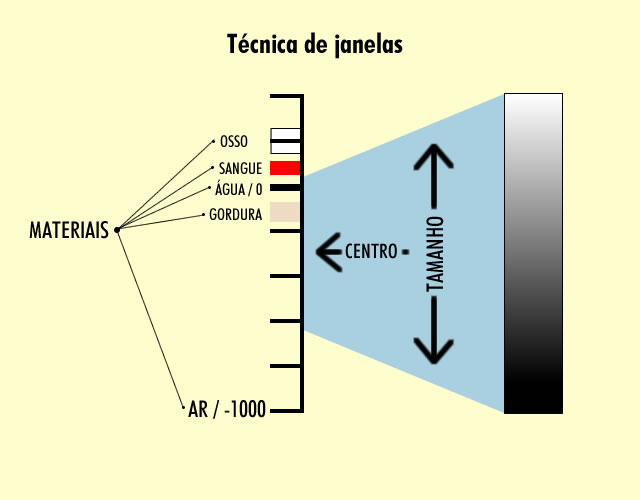
\includegraphics[height=3.0in]{imagens/tc_janela.jpg}
 \end{center}
 \caption{Exemplo de janela.}
 \label{fig:tc_janela}
\end{figure}

O uso de diferentes janelas em tomografia permite por exemplo o estudo dos ossos com distinção entre a cortical e a medular óssea ou o estudo de partes moles com a distinção, por exemplo, no cérebro entre a substância branca e a cinzenta. A mesma imagem pode ser mostrada com diferentes ajustes da janela, de modo a mostrar diferentes estruturas de cada vez. Não é possível usar um só ajuste da janela para ver, por exemplo, detalhes ósseos e de tecido adiposo ao mesmo tempo. Alguns valores comuns de janela estão na tab.~\ref{tab:janela}.

\begin{table}
 \caption{Valores comuns de janela para certos tipos de exame.}
% TODO: referencia
% TODO: fazer tabela
 \begin{center}
 \begin{tabular}{l|r|r}
 \hline
 	\textbf{Tecido a ser destacado} & \textbf{Largura da janela} & \textbf{Centro da janela} \\
 	Tórax na altura do mediastino & 500 & 39 \\
 	Pulmão & 850 & -500\\
 \hline
 \end{tabular}
 \end{center}
 \begin{description}
  \item Fonte: \citealt{oliveira}
 \end{description}
 \label{tab:janela}
\end{table}

\subsection{Padrão DICOM}

A introdução de imagens médicas digitais na década de 70 do século passado e o uso de computadores para processar estas imagens fizeram com que o American College of Radiology (ACR) e a National Electrical Manufacturers Association (NEMA) se juntassem para formar um comitê com o objetivo de criar um método padrão para a transmissão de imagens médicas e das informações associadas a elas.

Este comitê, constituído em 1983, publicou seu primeiro conjunto de padrões, chamado de ACR-NEMA, em 1985, e o segundo em 1988. Até a publicação dos padrões, a maioria dos equipamentos utilizava formatos proprietários para fazer o armazenamento e comunicação de imagens.

Embora as primeiras versões não tenham obtido êxito total na definição de um padrão comum, a terceira versão, publicada em 1993 sob o nome de DICOM (Digital Imaging and Communications in Medicine), conseguiu estabelecer uma forma padronizada de armazenamento e comunicação de imagens médicas e as correspondentes informações associadas.

Com os melhoramentos promulgados por esta terceira versão, o padrão estava pronto tanto para permitir transferência de imagens médicas em um ambiente com múltiplos fabricantes como também para facilitar o desenvolvimento e a expansão dos sistemas de armazenamento e de comunicação e a conexão com os sistemas de informação médica \cite{nema}.

Nos dias de hoje, a maioria dos fabricantes de equipamentos para aquisição de imagens médicas permite que os arquivos sejam exportados nesse formato, além dos formatos proprietários. Assim como a maioria dos softwares de processamento de imagens médicas também apresenta compatibilidade com esse formato.

\section{Segmentação}

Segmentação é a área do processamento de imagens que trata de isolar as regiões de interesse de uma imagem ou mudar a sua representação para facilitar a sua análise em determinada aplicação. Segmentação de imagens é tipicamente utilizada para localizar objetos e formas (curvas, linhas, etc) em imagens.

A segmentação de imagens não triviais é uma das tarefas mais difíceis no processamento de imagens. A precisão da segmentação determina o sucesso ou falha de um sistema de análise computadorizada \cite{gonzalez}.

Mas o processo de segmentação é enormemente facilitado quando o domínio das imagens do problema é bem conhecido e restrito. Desse forma permitindo que as técnicas de segmentação possam ser alteradas para trazer resultados mais satisfatórios no domínio do problema.

\subsection{Threshold Adaptativo}
\label{subsec:threshold}

Threshold é um dos métodos mais simples de segmentação de imagens. A partir de uma imagem em tons de cinza, o threshold pode ser usado para torná-la binária.

Durante o processo de threshold, os pixels são dividos em dois grupos, na forma mais simples de threshold, a divisão é feita dependendo apenas se o valor do pixel é maior ou menor que o valor de threshold. Então um grupo é colorido de preto e o outro de branco, tornando a imagem binária. A divisão dos grupos de pixels pode ser feita com base em mais de um valor de threshold, dessa forma os pixels são divididos entre os que estão dentro de um intervalo formado por 2 valores de threshold e os que não estão.

O parâmetro chave que determina a eficiência de um threshold é o valor de threshold usado. Diversos métodos existem para a escolha do valor de threshold, ele pode ser escolhido manualmente, ou por algum algoritmo que o compute, dependendo da imagem, esse tipo de threshold mais conhecido como thresolhd automático. Um método simples é escolher o valor da media ou da mediana. Geralmente esse algoritmo só irá atingir bons resultados se a imagem de entrada possuir pouco ruído e for uniforme. Uma abordagem um pouco mais sofisticada seria gerar o histograma da intensidade dos pixels da imagem e escolher como threshold o valor de vale.

A técnica de threshold adaptivo, que pode ser vista na fig.~\ref{fig:threshold}, consiste em escolher um valor inicial arbitrário de threshold ($T^0$), realizar o threshold e calcular o valor médio dos pixels acima ($\mu_{acima}$) e abaixo ($\mu_{abaixo}$) do valor de threshold. Então obter um novo threshold ($T^{i+1}$), de acordo com a equação~ \ref{equa:thresholdAdaptativo}. Com o novo threshold o processo se inicia novamente, e só para quando atingir a convergência, ou seja, o novo valor for igual ao antigo valor ($T^i = T^{i+1}$). Este algoritmo garante a convergência até um mínimo local.

\begin{equation}
 T^{i+1} = \frac{\mu_{acima}+\mu_{abaixo}}{2}
 \label{equa:thresholdAdaptativo}
\end{equation}

\begin{figure}[ht]
 \begin{center}
  \subfigure[Imagem original]{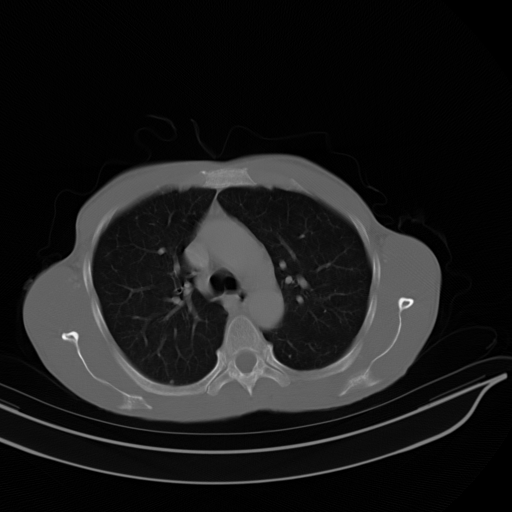
\includegraphics[width=2.9in]{imagens/TCpulmao.png}}
  \subfigure[Depois do threshold adaptativo]{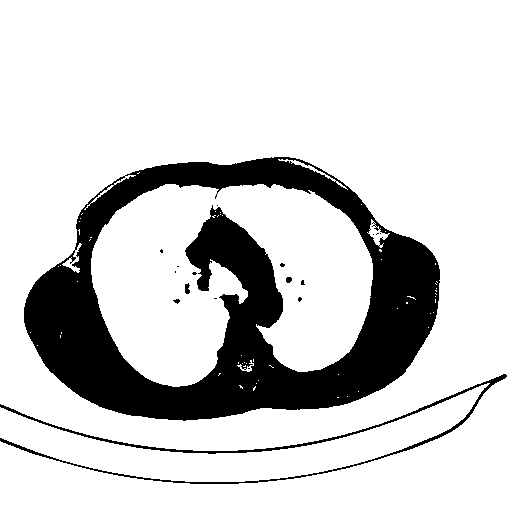
\includegraphics[width=2.9in]{imagens/TCpulmaoTHRESHOLDED.png}}
 \end{center}
 \caption{Imagem de TC original e após a aplicação de threshold adaptativo.}
 \label{fig:threshold}
\end{figure}

\section{Morfologia Matemática}

Morfologia é o estudo da forma. Em processamento de imagens, morfologia matemática é o nome que se dá a um conjunto de métodos, inicialmente desenvolvidos por Georges Matheron e Jean Serra  em 1964, que têm em comum o objetivo de estudar a estrutura geométrica de uma imagem.

A linguagem utilizada na morfologia matemática é a teoria dos conjuntos. Conjuntos na morfologia matemática representam objetos numa imagem. Por exemplo, o conjunto de todos os pixels pretos numa imagem binária é uma descrição morfologica completa da image. Em imagens binárias, os conjuntos em questão são membros do espaço dos inteiros bidimensional - 2D - $Z^2$, onde cada elemento do conjunto é uma tupla cujas coordenadas são as coordenadas de um pixel preto na image. Imagens em tons de cinza podem ser representadas como conjuntos cujos componentes estão em $Z^3$. Neste caso, dois componentes de cada elemento do conjunto se referem as coordenadas do pixel, e o terceiro corresponde ao valor do seu nível de cinza. Conjuntos em espaços dimensionais ainda mais elevados podem conter outros atributos da imagem, como cor ou componentes que variam com o tempo \cite{gonzalez}.

Então temos a morfologia binária que se aplica sobre imagens binárias e a morfologia cinza que se aplica a imagens em níveis de cinza. Uma operação morfológica binária é completamente determinada a partir da vizinhaça examinada ao redor do ponto central e do algoritmo utilizado, Já na morfologia cinza, na vizinhança de cada pixel, ou numa parte da vizinhança, é necessário conhecer o valor do pixel mais escuro, e o valor do mais claro. O valor do pixel resultando corresponde a uma combinação particular desses dois. Portanto o tamanho e a forma da vizinhança, as regiões de pesquisa dos valores máximo e minímo e o algoritmo utilizado, determinam uma operação de morfologia cinza \cite{facon}.

As operações fundamentais da morfologia matemática são a erosão e a dilatação. Essas operações necessitam do que chamamos de elementos estruturantes. Estes elementos, determinam quais pixels da imagem são retirados (no caso de uma erosão) ou quais são adicionados (no caso de uma dilatação) aos objetos. Elementos estruturantes são simplesmente imagens binárias em que um dos pontos é definido como centro. Como exemplos largamente utilizados podemos citar: um quadrado de 3x3 pixels (fig.~\ref{fig:ee_quadrado}), uma cruz definida pelo pontos {(-1,0),(0,-1),(0,0),(0,1),(1,0)} (fig.~\ref{fig:ee_cruz}) e um círculo de raio qualquer (fig.~\ref{fig:ee_circulo}).

\begin{figure}[ht]
 \begin{center}
  \subfigure[Quadrado (3x3))]{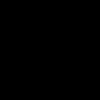
\includegraphics[width=1in]{imagens/ee_quadrado.png}\label{fig:ee_quadrado}}
  \hspace{1.5cm}
  \subfigure[Cruz (3x3)]{
\includegraphics[width=1in]{imagens/ee_cruz.png}\label{fig:ee_cruz}}
  \hspace{1.5cm}
  \subfigure[Círculo de raio 2 (5x5)]{
\includegraphics[width=1in]{imagens/ee_circulo.png}\label{fig:ee_circulo}}
 \end{center}
 \caption{Exemplos de elementos estruturantes.}
 \label{fig:elemento_estruturante}
\end{figure}

\subsection{Erosão e Dilatação}

Na erosão, o elemento estruturante é sobreposto à imagem em todas as posições possíveis. O pixel que fica na posição da origem do elemento estruturante é modificado da seguinte forma: se o elemento estiver em parte sobre o objeto e em parte sobre o fundo, o pixel que está na posição da origem passa a ser fundo. Ou seja, um pixel só pode permanecer no objeto se, quando a origem do elemento estruturante estiver sobre ele, todo o elemento estiver sobre o objeto, como podemos ver na fig.~\ref{fig:erosao}.
\\ \\
Efeitos da erosão:

\begin{itemize}
 \item Diminui as partículas;
 \item Elimina grãos de tamanho inferior ao tamanho do elemento estruturante;
 \item Aumenta os buracos;
 \item Separa grãos próximos.
\end{itemize}


Na dilatação o que muda é que quando o elemento está em parte sobre o fundo e em parte sobre o objeto, o seu centro passa a ser objeto, como vemos na fig.~\ref{fig:dilatacao}. Isto aumenta o tamanho do objeto, como o nome dilatação sugere.
\\ \\
Efeitos da dilatação:

\begin{itemize}
 \item Aumenta as partículas;
 \item Preenche pequenos buracos;
 \item Conecta grãos próximos.
\end{itemize}

\begin{figure}[ht]
 \begin{center}
  \subfigure[Imagem Original]{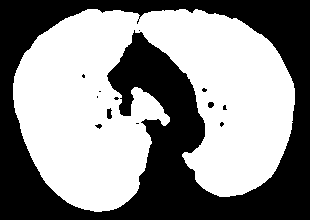
\includegraphics[width=2.9in]{imagens/afterHoleFilling.png}}
  \\
  \subfigure[Dilatação]{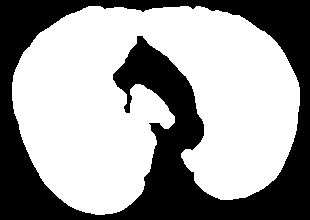
\includegraphics[width=2.9in]{imagens/dilatacao.png}\label{fig:dilatacao}}
  \subfigure[Erosão]{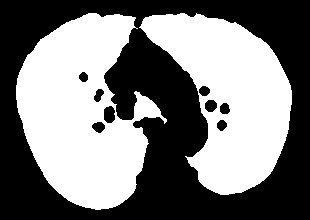
\includegraphics[width=2.9in]{imagens/erosao.png}\label{fig:erosao}}
 \end{center}
 \caption{Imagem de TC após passar por threshold adaptativo e limpeza, submetida a dilatação e erosão utilizando como elemento estruturante um círculo de raio 3 pixels.}
 \label{fig:erosao_dilatacao}
\end{figure}

\subsection{Abertura e Fechamento}

Erosão e dilatação podem corrigir defeitos numa imagem com furos, conexões. Porém, o objeto alterado por essas operações não mantém o mesmo tamanho. A erosão reduz e a dilatação aumenta. Com a abertura e o fechamento binários, podemos manter aproximadamente as características de forma e tamanho do objeto.

A abertura é obtida através da erosão, seguida de uma dilatação da imagem resultante com o mesmo elemento estruturante. Esta operação é capaz de eliminar pequenas partículas inferiores em tamanho ao elemento estruturante quase sem modificar o tamanho das outras entidades, além de nivelar os contornos pelo interior, como podemos ver na fig.~\ref{fig:abertura}.

Já o fechamento é o inverso; dilatação, seguida de erosão. Ele conecta partículas próximas, suaviza as bordas pelo exterior e preenche os buracos inferiores em tamanho em relação ao elemento estruturante que estejam no interior das partículas, visto na fig.~\ref{fig:fechamento}.

\begin{figure}[ht]
 \begin{center}
  \subfigure[Imagem Original]{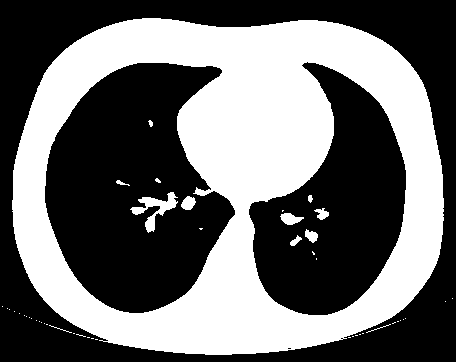
\includegraphics[width=2.9in]{imagens/afterThreshold.png}}
  \\
  \subfigure[Abertura]{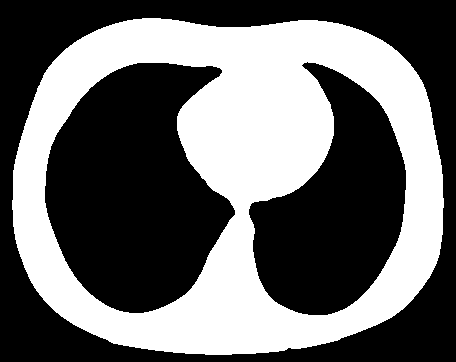
\includegraphics[width=2.9in]{imagens/abertura.png}\label{fig:abertura}}
  \subfigure[Fechamento]{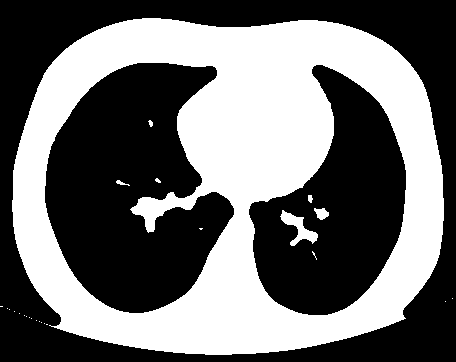
\includegraphics[width=2.9in]{imagens/fechamento.png}\label{fig:fechamento}}
 \end{center}
 \caption{Imagem de TC após passar por threshold adaptativo, submetida a abertura e fechamento utilizando como elemento estruturante um círculo de raio 6 pixels.}
 \label{fig:abertura_fechamento}
\end{figure}

\section{Extração de características de texturas}

O sistema de visão humano percebe uma cena como sendo variações de intensidade e cor, a imagem toda ou as partes dela que formam certos padrões repetitivos, são chamadas de textura. Numa imagem de textura, um conjunto estatístico ou de atributos, varia lentamente ou se mantém quase periódico. Estes atributos, os quais são repetitivos ou quase, dominam as texturas de uma cena.

Uma textura é uma junção de subpadrões que se repetem, que seguem um conjunto de regras de posicionamento bem definido. Estes subpadrões são feitos de unidades mais básicas, chamadas de primitivas. Esta caracterização de texturas é principalmente aplicável a texturas determinísticas, como por exemplo, linhas, tabuleiro de dama, etc. Existem imagens, como imagens de satélite da superfície terreste, que aparentemente não possuem esses padrões básicos que são repetidos ao longo do padrão mais abrangente \cite{acharya}.

Uma imagem que seja uma textura, pode então ser toda reduzida num conjunto de características, também chamado de vetor de características. Essa transformação se chama extração de características. Se as características extraídas forem cuidadosamente escolhidas é esperado que o conjunto de características represente toda a informação relevante da textura.

Uma primitiva é um conjunto conectado de pixels, caracterizado por um conjunto de atributos. A primitiva mais simples é um único pixel com seu atributo de nível de cinza. Um conjunto de pixels conectado que possui o mesmo nível de cinza ou que possui a mesma direção de borda forma uma primitiva. Outros atributos locais podem ser considerados para se definir uma primitiva. Outros atributos incluem a medida de regiões conectadas e a homogeneidade da sua propriedade local. Primitivas podem ser geradas a partir de imagens por vários filtros de vizinhança \cite{acharya}.

\subsection{Matriz de co-ocorrência}

Matriz de co-ocorrência é um dos métodos de processamento de imagens utilizado para caracterizar texturas. Ele descreve uma imagem, ou uma região de interesse na imagem, em termos da relação entre os valores dos pixels com os valores dos pixels vizinhos.

Uma matriz de co-ocorrência é definida a partir de uma imagem como sendo a distribuição dos valores co-ocorrentes num dado deslocamento. Matematicamente, a matrix de co-ocorrência $C$ é definida a partir de uma imagem $I$ de $N x M$, parametrizada com um deslocamento de ($\Delta{}x,\Delta{}y$), como podemos ver abaixo:

\begin{equation}
 C(i,j)=\sum_{p=1}^n\sum_{q=1}^m
 \cases{
	1, & $\mbox{se }I(p,q)=i\mbox{ e }I(p+\Delta{}x,q+\Delta{}y)=j$\cr
	0, & $\mbox{senão}$\cr
 }
\end{equation}

Para poder ser utilizada, a matriz de co-ocorrência precisa ser normalizada, que poder ser obtida dividindo cada elemento da matriz pelo número total de pares de pixel.

Percebemos que o deslocamento ($\Delta{}x,\Delta{}y$) faz com que a matriz de co-ocorrência seja sensível a rotação. Dessa forma, uma rotação da imagem diferente de 180 graus irá resultar numa matriz de co-ocorrência diferente para uma mesma imagem (rotacionada). Isso é raramente desejado nas aplicações em que a matriz de co-ocorrência é utilizada, portanto a matriz de co-ocorrência é geralmente utilizada a partir da média em cada valor da matriz para um conjunto de deslocamentos que variam até 180 graus com uma mesma distância entre eles (por exemplo 0, 45, 90 e 135 graus) para não ser influenciada pela rotação.

\subsection{Características de Haralick}

\citealt{Haralick} sugeriu um total de 14 características que podem ser computadas diretamente da matriz de co-ocorrência, as quais podem ser utilizadas para classificar imagens de textura. Abaixo estão descritas algumas delas.

Considere N como sendo o número de níveis de cinza da matriz de co-ocorrência e.

A Energia, também conhecida como segundo momento angular, avalia a uniformidade textural em uma imagem. A fórmula que descreve a energia pode ser vista na equação~\ref{equa:hara-energia}.

\begin{equation}
 \sum_{i=0}^{N-1}\sum_{j=0}^{N-1} C(i,j)^2
 \label{equa:hara-energia}
\end{equation}

A Entropia mede a desordem em uma imagem, ou seja, o grau de dispersão de níveis de cinza. Ela é calculada como na equação \ref{equa:hara-entropia}.

\begin{equation}
 -\sum_{i=0}^{N-1}\sum_{j=0}^{N-1} C(i,j) \; log(C(i,j))
 \label{equa:hara-entropia}
\end{equation}

O contraste, mede a presença de transição abrupta de níveis de cinza (bordas) na imagem. Ele é definido como:

\begin{equation}
 \sum_{x=0}^{N-1} x^2 \left\{\sum_{i=0}^{N-1}\sum_{j=0}^{N-1} C(i,j)\right\},|i - j| = x
 \label{equa:hara-contraste}
\end{equation}

A homogeneidade local, também conhecido como momento diferencial inverso, como o próprio nome sugere, mede a homogeneidade da imagem. Sua fórmula é:

\begin{equation}
 \sum_{i=0}^{N-1}\sum_{j=0}^{N-1} \frac{1}{1 + (i - j)^2} \;C(i,j)
 \label{equa:hara-homogeneidade}
\end{equation}

A correlação mede a dependência linear de um nível de cinza em relação aos vizinhos. Ela é calculada como na equação~\ref{equa:hara-correlação}.

\begin{equation}
 \frac{\sum\limits_{i=0}^{N-1}\sum\limits_{j=0}^{N-1} i j\; C(i,j) - \mu_{i}^2}{\sigma_{i}^2}
 \label{equa:hara-correlação}
\end{equation}

Onde $\mu_{i}$ representa a média ponderada, como definido na equação~\ref{equa:hara-media}. Por causa da simetria da matriz de co-ocorrência, não é necessário calcular a média ponderada de $\mu_{j}$. Já $\sigma_{i}$ representa o desvio padrão, como na equação~\ref{equa:hara-desvio}, que também se beneficia da simetria.

\begin{equation}
 \sum_{j=0}^{N-1}\sum_{i=0}^{N-1} i \cdot C(i, j)
 \label{equa:hara-media}
\end{equation}

\begin{equation}
 \sum_{j=0}^{N-1}\sum_{i=0}^{N-1} (i - \mu_{i})^2 \cdot C(i, j)
 \label{equa:hara-desvio}
\end{equation}

Além dessas características, também estão definidas em \cite{Haralick}: soma dos quadrados, soma da média, soma da variância, soma da entropia, variância diferencial, entropia diferencial, medida de informação da correlação e coeficiente de correlação máxima.
